\section{Parte práctica: procesamiento de la señal \senal}
\label{sec:practico}

\subsection{Datos y parámetros del radar}
\label{sec:parametros}
La señal asignada (\texttt{signal\_\senal.csv}) es una detección simulada de radar con 100 momentos de muestreo, es decir, 100 pulsos consecutivos, con entre 2 y 10 blancos de rangos y velocidades desconocidos \cite{consigna}. Cada pulso tiene 2000 muestras complejas (I/Q) de tiempo rápido, que cubren de 15 m a 30 km con un paso de $c\,t_s/2 = 15 \, [m]$. Los datos se ordenan en una matriz de $100 \times 2000$: las filas son el \textbf{tiempo lento} (pulso a pulso, separados una PRI) y las columnas el \textbf{tiempo rápido} (rango). Se procesaron en Python (\texttt{numpy}, \texttt{scipy}, \texttt{matplotlib}) a partir del código provisto por la cátedra \cite{codigo_catedra}. El script \texttt{practico/tp5\_radar.py} reproduce todos los resultados con \texttt{python tp5\_radar.py \senal}.

\begin{table}[H]
    \centering
    \footnotesize
    \caption{Parámetros del radar simulado \cite{codigo_catedra} y magnitudes derivadas.}
    \label{tab:parametros}
    \begin{tabular}{|l|r||l|r|}
        \hline
        \textbf{Parámetro} & \textbf{Valor} & \textbf{Magnitud derivada} & \textbf{Valor} \\
        \hline
        Frecuencia portadora $f_c$ & 1,3 GHz & Longitud de onda $\lambda = c/f_c$ & 23,1 cm \\
        Frecuencia de muestreo $f_s$ & 10 MHz & Paso en rango $c/(2f_s)$ & 15 m \\
        Duración del chirp $T_p$ & 10 $\mu$s & Resolución en rango $c/(2B)$ & 75 m \\
        Ancho de banda del chirp $B$ & 2 MHz & Producto $BT$ (ganancia de compresión) & 20 (13 dB) \\
        PRF & 1500 Hz & PRI & 666,7 $\mu$s \\
        Recuperación del transmisor $T_e$ & 5 $\mu$s & Rango mínimo $(T_p/2 + T_e)c/2$ & 1,5 km \\
        Pulsos $N_p$ & 100 & Rango no ambiguo $c(PRI - T_p - T_e)/2$ & 97,75 km \\
        Ventana de rango & 30 km & Intervalo de velocidad no ambigua $\pm \lambda\,PRF/4$ & $\pm 86{,}5$ m/s \\
        \hline
    \end{tabular}
\end{table}

\subsection{Operaciones realizadas}
\label{sec:operaciones}
La \autoref{fig:flujo} resume la cadena de procesamiento, que sigue el diagrama de la consigna \cite{consigna}.

\begin{figure}[H]
    \centering
    \resizebox{\textwidth}{!}{%
    \begin{tikzpicture}[font=\footnotesize, node distance=0.5cm and 0.6cm,
        b/.style={draw, thick, rounded corners=2pt, fill=blue!8, minimum height=0.9cm, text width=2.1cm, align=center},
        f/.style={-{Stealth}, thick}]
        \node[b] (raw) {Datos crudos $100 \times 2000$};
        \node[b, right=of raw] (mf) {Filtro apareado (compresión)};
        \node[b, right=1.0cm of mf, fill=orange!12] (sti) {STI SC $1 + z^{-1}$};
        \node[b, above=of sti, fill=orange!12] (mti) {MTI SC $1 - z^{-1}$};
        \node[b, below=of sti, fill=orange!12] (dc) {MTI DC $1 - 2z^{-1} + z^{-2}$};
        \node[b, right=of mti, fill=green!10] (dop) {Filtrado Doppler (DFT en tiempo lento)};
        \node[b, right=of sti, fill=green!10] (cfar) {CFAR y cruces por cero};
        \node[b, right=of dop, fill=purple!10] (vel) {Rango y velocidad de blancos móviles};
        \node[b, right=of cfar, fill=purple!10] (rng) {Rango de los blancos (móviles y fijos)};
        \draw[f] (raw) -- (mf); \draw[f] (mf) -- (sti); \draw[f] (mf.east) -- ++(0.4,0) |- (mti); \draw[f] (mf.east) -- ++(0.4,0) |- (dc);
        \draw[f] (mti) -- (dop); \draw[f] (dop) -- (vel); \draw[f] (sti) -- (cfar); \draw[f] (cfar) -- (rng);
        \draw[f] (mti.east) -- ++(0.25,0) |- (cfar); \draw[f] (dc.east) -- ++(0.25,0) |- (cfar);
    \end{tikzpicture}}
    \caption{Cadena de procesamiento implementada.}
    \label{fig:flujo}
\end{figure}

\textbf{1. Compresión con filtro apareado.} Se genera el chirp de referencia $s(t) = \mathrm{rect}(t/T_p) \, e^{j\pi (B/T_p) t^2}$ y el filtro apareado $h(t) = s^*(-t)$ (\autoref{sec:filtro_apareado}). Cada pulso recibido $x_p[n]$ se convoluciona con $h$ mediante la FFT (función \texttt{fastconv} de la cátedra, con relleno de ceros a la potencia de 2 siguiente):
\begin{equation}
    y_p[n] = \sum_k x_p[k] \, h[n - k] = \mathrm{IFFT}\{ X_p(f) \, S^*(f) \}
\end{equation}
La salida de la convolución tiene $2 \cdot 2000 - 1$ muestras. Se conservan las 2000 centrales, a partir del índice $(N_h - 1)/2$, para que el pico de cada eco coincida con su rango. La alineación se verificó con un eco sintético a 10 km, cuyo pico comprimido aparece exactamente en $10{,}005$ km, la celda de 15 m que lo contiene.

\textbf{2. Canceladores en tiempo lento.} Operan sobre la señal comprimida, celda de rango por celda de rango, entre pulsos consecutivos:
\begin{align}
    \text{MTI simple cancelador:} \quad & y_p = x_p - x_{p-1}, & H(z) &= 1 - z^{-1}, & |H(f_D)| &= 2\left|\sin(\pi f_D / PRF)\right| \\
    \text{STI simple cancelador:} \quad & y_p = x_p + x_{p-1}, & H(z) &= 1 + z^{-1}, & |H(f_D)| &= 2\left|\cos(\pi f_D / PRF)\right| \\
    \text{MTI doble cancelador:} \quad & y_p = x_p - 2x_{p-1} + x_{p-2}, & H(z) &= (1 - z^{-1})^2, & |H(f_D)| &= 4\sin^2(\pi f_D / PRF)
\end{align}
con $f_D = 2v_r/\lambda$. El MTI es un filtro pasaaltos en Doppler: anula los ecos fijos (clutter y blancos detenidos) y deja pasar los móviles. El doble cancelador tiene un nulo más ancho y profundo alrededor de $f_D = 0$, mejor para clutter con dispersión Doppler, pero atenúa más a los blancos lentos. El STI es pasabajos: refuerza los ecos fijos y anula los blancos cuya $f_D$ se acerca a $\pm PRF/2$. Todos se repiten cada $PRF$: un blanco con velocidad $v_b = k \lambda \, PRF/2 = k \cdot 173 \, [m/s]$ (velocidad ciega) es cancelado por el MTI como si estuviera fijo (\autoref{fig:canceladores}).

\begin{figure}[H]
    \centering
    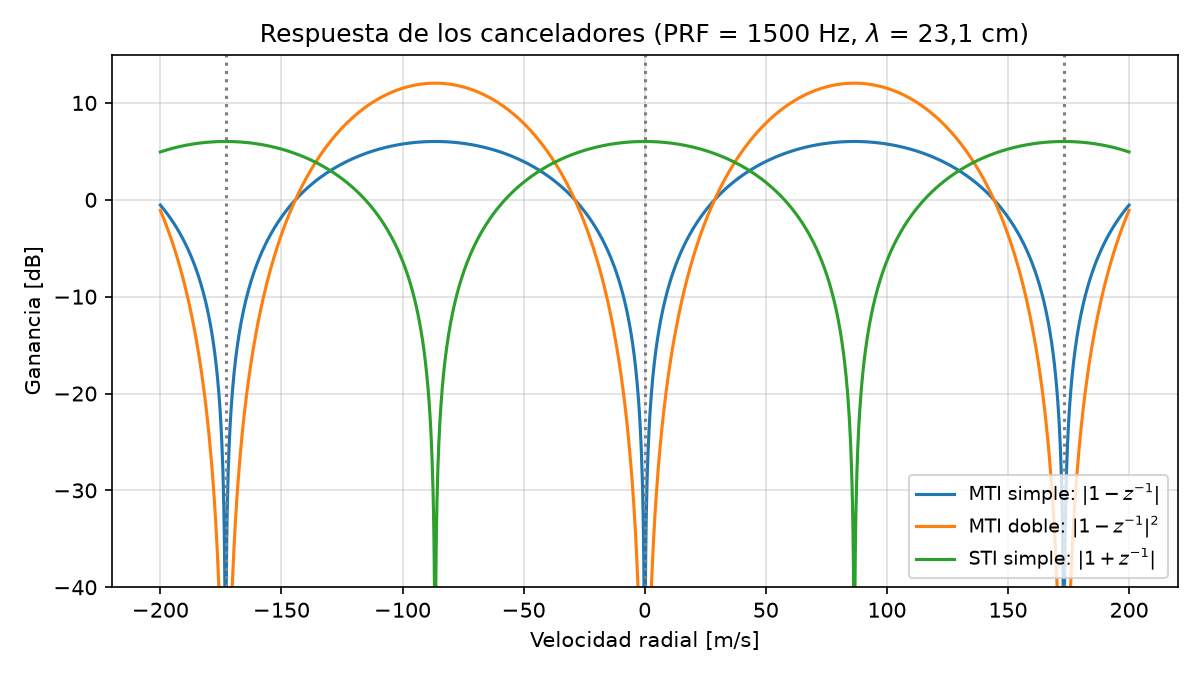
\includegraphics[width=0.78\textwidth]{teoria/respuesta_canceladores.png}
    \caption{Respuesta en frecuencia de los canceladores en función de la velocidad radial. Las líneas punteadas marcan la velocidad nula y las velocidades ciegas $\pm 173 \, [m/s]$. Elaboración propia.}
    \label{fig:canceladores}
\end{figure}

\textbf{3. Ventana CFAR y umbral.} Se usa un detector CA-CFAR (\textit{cell averaging}): para cada celda bajo prueba se estima la potencia de ruido como el promedio de $N_R$ celdas de referencia, dejando $N_G$ celdas de guarda a cada lado para que el propio blanco no eleve la estimación \cite{apunte, richards}. Implementado como convolución con la ventana $w$ (\autoref{fig:ventana_cfar}),
\begin{equation}
    \hat{P}[n] = \sum_k w[k] \, |y[n-k]|^2,
    \qquad
    w[k] = \begin{cases} 1/N_R & \text{celdas de referencia} \\ 0 & \text{celdas de guarda y celda bajo prueba} \end{cases}
\end{equation}
y se declara detección cuando $|y[n]|^2 > \alpha \, \hat{P}[n]$. Para ruido gaussiano complejo detectado en potencia, la $P_{fa}$ de diseño fija el factor del umbral \cite{richards}:
\begin{equation}
    P_{fa} = \left(1 + \frac{\alpha}{N_R}\right)^{-N_R}
    \quad \Rightarrow \quad
    \alpha = N_R \left( P_{fa}^{-1/N_R} - 1 \right)
\end{equation}
Se adoptaron $N_R = 64$ celdas de referencia (32 de cada lado, 480 m) y $N_G = 8$ celdas de guarda por lado (120 m), con $P_{fa} = 10^{-6}$:
\begin{itemize}
    \item $\alpha = 15{,}4$, que en amplitud corresponde a una \textbf{ganancia del umbral de $\sqrt{\alpha} = 3{,}93$} sobre el valor eficaz del ruido estimado.
    \item Las celdas de guarda cubren el lóbulo principal del eco comprimido ($\pm 75$ m, 5 celdas) y sus primeros lóbulos laterales ($\pm 110$ m), para que el blanco no se cuente como ruido.
    \item El ejemplo de la consigna usa 200 celdas de referencia (1,5 km por lado). Con esa ventana se verificó enmascaramiento: un blanco fuerte dentro de la ventana de otro eleva su umbral y lo oculta (con la señal 2, el blanco fijo de 22,02 km quedaba oculto por los de 20,2--20,3 km). La ventana de 64 celdas reduce ese efecto con una pérdida CFAR moderada.
    \item En los extremos del vector de rango hay menos celdas de referencia; el promedio se normaliza por las celdas disponibles para que el umbral no caiga artificialmente en los bordes.
\end{itemize}

\begin{figure}[H]
    \centering
    \includegraphics[width=0.55\textwidth]{\figdir/03_ventana_cfar.png}
    \caption{Ventana CFAR utilizada: 64 celdas de referencia (32 por lado, con valor $1/64$), 8 celdas de guarda por lado y la celda bajo prueba en el centro (valor 0).}
    \label{fig:ventana_cfar}
\end{figure}

\textbf{4. Detección por cruces por cero.} La función $d[n] = \mathrm{sign}(|y[n]| - V_T[n])$ vale $+1$ donde la señal supera el umbral. Su diferencia, $\Delta d[n] = d[n+1] - d[n]$ (funciones \texttt{numpy.sign} y \texttt{numpy.diff}), vale $+2$ donde comienza una detección y $-2$ donde termina. El rango del blanco es el del máximo de $|y|$ dentro de cada intervalo. Las detecciones a menos de 150 m (dos celdas de resolución) se agrupan, porque corresponden al mismo eco y sus lóbulos laterales. Se descartan las celdas por debajo del rango mínimo de 1,5 km.

Los gráficos CFAR usan, como pide la consigna, un único momento de muestreo: los pulsos $t_0$ y $t_1$ para los canceladores simples y $t_0$, $t_1$ y $t_2$ para el doble. Para una lista de detecciones más robusta se aplica además el CFAR a la potencia de la salida de cada cancelador promediada sobre todos los pulsos (integración no coherente).

\textbf{5. Filtrado Doppler.} La señal del MTI simple cancelador (99 pulsos $\times$ 2000 celdas) se multiplica, transpuesta, por la matriz de la DFT de $m = 99$ puntos \cite{consigna}:
\begin{equation}
    \mathbf{Y} = (\mathbf{MTI}_{SC})^T \, \mathbf{F_D},
    \qquad
    F_D[r, c] = e^{-j 2\pi r c / m}, \quad r, c = 0, \dots, m-1
\end{equation}
Cada fila de $\mathbf{Y}$ es el espectro Doppler de una celda de rango, que integra coherentemente los 99 pulsos. La columna $k$ (centrada con \texttt{fftshift}) corresponde a $f_D = (k - m/2) \, PRF/m$ y a la velocidad radial $v_r = f_D \lambda/2$, con una resolución de $\lambda \, PRF/(2m) = 1{,}75 \, [m/s]$. Con la convención de fase del simulador ($e^{-jk \, 2R}$), una velocidad positiva corresponde a un blanco que se acerca y una negativa, a uno que se aleja. Las velocidades solo son únicas dentro de $\pm 86{,}5 \, [m/s]$: un blanco más rápido aparece replegado (\textit{aliasing}).

Para obtener la lista de blancos, sobre el mapa rango-Doppler se aplica el mismo CA-CFAR en rango para cada frecuencia Doppler. Para esa detección se pondera el tiempo lento con una ventana de Hamming, que baja los lóbulos laterales Doppler de $-13$ a $-43$ dB; sin ella, junto a cada blanco de unos 40 dB de SNR aparecían decenas de detecciones falsas en otras velocidades. Esta detección tiene dos ventajas: la integración coherente de 99 pulsos (casi 20 dB de ganancia) y la separación de blancos cercanos en rango pero con distinta velocidad, que ya no se enmascaran entre sí.

\textbf{6. Clasificación de los blancos.} Las detecciones se combinan con estos criterios:
\begin{itemize}
    \item \underline{Blanco móvil:} detección rango-Doppler confirmada por algún cancelador a menos de 150 m, o con SNR de al menos 20 dB. Su velocidad es la del máximo Doppler.
    \item \underline{Residuo:} una detección en la misma celda de rango que otra más de 20 dB más fuerte corresponde a la dispersión Doppler del blanco fuerte, por la fluctuación de su RCS entre pulsos, y no se cuenta como blanco.
    \item \underline{Falsa alarma:} una detección débil (SNR menor que 20 dB) que ningún cancelador confirma. En las señales 1, 2 y de ejemplo aparecen las mismas tres (1,5, 6,2 y 13,7 km), lo que indica que las simulaciones comparten la realización del ruido.
    \item \underline{Blanco fijo:} detección del STI integrado donde la salida del STI supera a la del MTI en más de 10 dB, porque el MTI cancela casi toda su energía.
\end{itemize}

\textbf{Validación.} El procedimiento se probó con la señal de ejemplo (\texttt{signal\_example.csv}). Se detectan tres blancos móviles en 10,02, 15,02 y 20,01 km, que coinciden con los de la Figura 5 de la consigna (9,95, 14,97 y 19,93 km), y un blanco fijo en 18,02 km, que solo aparece sin cancelar.
